\section{Document-Driven web Development Process}
\label{sec:document_driven_web_development_process}
The process to build a web application based on x-commerce toolkit consists of the following four steps: models schemas definition, HTTP RESTful API definition, UI components definition and UI components assembly.
\subsection{1st step - Model schemas definition}
A description of entities, properties, relations and data access policies are defined as JSON documents.
\newline
The models of e-commerce are many and are expected to grow further with the integration and implementation of new services. For the moment there are 30 models. Loopback in the definition of each model is done by filling in a JSON file where declare properties that interest us. In the following are the main models of x-commerce:
\begin{itemize}
\item \emph{product}: the model has the properties we are specifying the property of a product which interest, for which:
\begin{itemize}
\item a product has a title string (we are also saying that this field is required);
\item a product has a description string;
\item a product has a price of type Number, etc..
\end{itemize}
The model has also produced the “relations”. This field identifies relatiosn current model (“product”) with other models such as:
\begin{itemize}
\item a product has a relationship with the model “Image” type “many”. This report was modeled because the product has a lot of pictures;
\item a product has the relationship with the model “Comments” type “many” because a product has many comments or reviews, etc..
\item it is possible also specify “acls (access control lists)” to control access to the system. Specifying who can do what with a JSON file, you can have in a transparent way all security mechanisms.
\end{itemize}
\begin{lstlisting}[language=json]
{
  "name": "Product",
  "properties": {
    "title": {
      "type": "String",
      "required": true
    },
    "description": {
      "type": "String"
    },
    "price":  {
      "type": "Number"
    },
    ...........
  },
  "relations": {
    "images": {
          "type": "hasMany",
          "model": "Image"
        },
    "comments": {
      "type": "hasMany",
      "model": "Comment"
    },
    "collections": {
      "type": "hasAndBelongsToMany",
      "model": "Collection",
      "through": "CollectionProduct"
    },
    "options": {
      "type": "hasMany",
      "model": "ProductOption"
    },
    "product_type": {
      "type": "belongsTo",
      "model": "ProductType"
    },
    "variants": {
      "type": "hasMany",
      "model": "ProductVariant"
    },
    "vendor": {
      "type": "belongsTo",
      "model": "Vendor",
    },
    ...........
  }
}
\end{lstlisting}
\item \emph{customers}: this time there are two new things:
\begin{itemize}
\item the presence of \emph{acls}: in this case acls block all calls except “find” and count” that can call all;
\item note the presence of the \emph{“base”: “Users”}: “Users” is a model of loopback that is offered for free. This model brings back all funtionality related to login, sign up, forgot etc.. “Customer” model extends the “Users” loopback - and in this way the “Customer” legacy capabilities and therefore all methods APIs and “Users” including methods for login and logout.
\begin{lstlisting}[language=json]
{
  "name": "Customer",
  "base": "User",
  "properties": {
    "first_name": {
      "type": "String",
      "required": true
    },
    "last_name": {
      "type": "String",
      "required": true
    },
    "date_of_birth" : {
      "type": "Date"
    },
    "gender": {
      "type": "String",
      "enum": ["M", "F"]
    },
    "email": {
      "type": "String",
      "required": true
    },
    ...........
  },
  "acls": [
    {
      "principalType": "ROLE",
      "principalId": "$everyone",
      "permission": "ALLOW",
      "property": "find"
    },
    {
      "principalType": "ROLE",
      "principalId": "$everyone",
      "permission": "ALLOW",
      "property": "count"
    },
    ...........
  ]
}
\end{lstlisting}
\end{itemize}
\end{itemize}

Each file JSON is also accompanied by a js file. This file is used to define the so-called “hooks” or the methods to define new APIs customized. These new APIs are added to the API generated by the JSON file.
\begin{lstlisting}[language=javascript]
module.exports = function (Product) {
};
\end{lstlisting}
Inside the function offered to extend the API, it is possbile to define new APIs. The name of the API is declared costs as follows:
\begin{lstlisting}[language=javascript]
module.exports = function (Product) {
  Product.remoteMethod('generate_variants', {
    accepts: { arg: 'product_id', type: 'string', required: true },
    returns: { arg: 'variants', type: 'Array' },
    http: { verb: 'get', path:'/generate' }
  });
};
\end{lstlisting}
The remote method remote method takes two parameters:
\begin{itemize}
\item name of the method to execute the call of the API in question - In this way, the method name is “generate\_variants”. This method will be executed when it is called api: “/api/Products/generate”;
\item as the second parameter, the remote method accepts a JSON object consisting of key-value pairs:
\begin{itemize}
\item “accepts”: indicates the input parameters ie parameters selling sent the body of the request. In this case the input parameter is the only one and is of type String and is required.
\item “returns”: It indicates what type is the response;
\item “http”: This is a parameter that defines url API. Therefore, url for call the generate API is: “/api/Products/generate”. When you call this API, it is invoked and executed the remote method declared as the first parameter. The remote method must be defined freely by the programmer.
\end{itemize}
\end{itemize}
Therefore, the complete example to define new APIs via remote methods, which are not generated by default from JSON file, is the following:
\begin{lstlisting}[language=javascript]
module.exports = function (Product) {
  Product.generate_variants = function (product_id, callback) {
    // to do anythings. Genreate a result
    callback(null, result);
  };

  Product.remoteMethod('generate_variants', {
    accepts: { arg: 'product_id', type: 'string', required: true },
    returns: { arg: 'variants', type: 'Array' },
    http: { verb: 'get', path:'/generate' }
  });
};
\end{lstlisting}
\subsection{2nd step - HTTP RESTful API definition}
CRUD operations on models are automatically generated by the web framework (on the basis of input JSON documents) and further custom actions can be defined. Following models of e-commerce are:
\begin{itemize}
\item \emph{products}: as already mentioned, it is the main model of the project. The properties of this model are easy to imagine because it's property that we all seek when we buy a product or a fine. So a product has:
\begin{itemize}
\item \emph{title}: type string;
\item \emph{description}: type string;
\item \emph{price}: type Number;
\item \emph{compare\_at\_price}: type Number - This data is related to the “free” product and is used to show a reduced price to the client-side;
\item \emph{is\_charge\_taxes}: type Boolean - This data is used to load the order of taxes or not. Some customers may be absent from paying taxes;
\item \emph{sku}: type String - stock keeping unit or SKU - is a number or string of alpha and numeric characters that uniquely identify a product;
\item \emph{barcode}: type String - is the small image of lines (bars) and spaces that is affixed to retail store items, identification cards, and postal mail to identify a particular product number, person, or location;
\item \emph{track\_quantity}: type Boolean - used to keep track of the amount of products.
\item \emph{quantity}: type Number;
\item \emph{sell\_after\_purchase}: type Boolean;
\item \emph{unit\_measure\_weight}: type String;
\item \emph{weight}: type Number;
\item \emph{is\_published}: type Boolean;
\item \emph{published\_at}: type Date;
\item \emph{tags}: type Array of String
\end{itemize}
\item \emph{article}:
\begin{lstlisting}[language=json]
{
  "name": "Article",
  "properties": {
    "title": { "type": "string", "required": true },
    "subtitle": { "type": "string" },
    "summary": { "type": "string" },
    "content": { "type": "string" },
    "created_at": { "type": "date" },
    "updated_at": { "type": "date" },
    "published_at": { "type": "date" },
    "tags": { "type": ["string"] }
},
"relations": {
"author": { "type": "belongsTo", "model": "Manager" },
"category": { "type": "belongsTo", "model": "Category" },
    "images": {
      "type": "hasMany",
      "model": "Image",
      "foreignKey": "article_id"

    }
  }
}
\end{lstlisting}
\item \emph{collection\_filters}:
\begin{lstlisting}[language=json]
{
  "name": "CollectionFilter",
  "properties": {
    "name": {
      "type": "String"
    },
    "type": {
      "type": "String"
    },
    "relation": {
      "type": "String"
    },
    "value": {
      "type": "String"
    }
  }
}
\end{lstlisting}
\item \emph{collections}:
\begin{lstlisting}[language=json]
{
  "name": "Collection",
  "properties": {
    "title": {
      "type": "String",
      "required": true
    },
    "description": {
      "type": "String"
    },
    "is_published": {
      "type": "Boolean"
    },
    "published_at": {
      "type": "Date"
    }
  },
  "validations": [],
  "relations": {
    "images": {
      "type": "hasMany",
      "model": "Image",
    },
    "products": {
      "type": "hasAndBelongsToMany",
      "model": "Product",
      "through": "CollectionProduct"
    }
  }
}
\end{lstlisting}
\item \emph{comment\_replies}:
\begin{lstlisting}[language=json]
{
  "name": "CommentReply",
  "properties": {
    "text": {
      "type": "string"
    },
    "created_at": {
      "type": "date"
    }
  },
  "validations": [],
  "relations": {
    "author": {
      "type": "belongsTo",
      "model": "Customer",
      "foreignKey": "author_id"
    }
  }
}
\end{lstlisting}
\item \emph{comments}:
\begin{lstlisting}
{
  "name": "Comment",
  "properties": {
    "title": {
      "type": "String"
    },
    "text": {
      "type": "String"
    },
    "created_at": {
      "type": "Date"
    }
  },
  "relations": {
    "author": {
      "type": "belongsTo",
      "model": "Customer"
    },
    "replies": {
      "type": "hasMany",
      "model": "CommentReply"
    }
  }
}
\end{lstlisting}
\item \emph{coupons}:
\begin{lstlisting}
{
  "name": "Coupon",
  "properties": {
    "name": {
      "type": "String",
      "required": true
    },
    "description": {
      "type": "String"
    },
    "discount": {
      "type": "Number",
      "required": true
    },
    "code": {
      "type": "String",
      "required": true
    },
    "date_from": {
      "type": "Date"
    },
    "date_to": {
      "type": "Date"
    }
  },
  "relations": {
    "order": {
      "type": "belongsTo",
      "model": "Order",
    }
  }
}
\end{lstlisting}
\item \emph{customers}:
\begin{lstlisting}
{
  "name": "Customer",
  "base": "User",
  "properties": {
    "first_name": {
      "type": "String",
      "required": true
    },
    "last_name": {
      "type": "String",
      "required": true
    },
    "date_of_birth" : {
      "type": "Date"
    },
    "gender": {
      "type": "String",
      "enum": ["M", "F"]
    },
    "email": {
      "type": "String",
      "required": true
    },
    ........
  },
  "relations": {
    "shipping_addresses": {
      "type": "hasMany",
      "model": "Address"
    },
    "wishlists": {
      "type": "hasMany",
      "model": "Wishlist"
    }
  }
}
\end{lstlisting}
\item \emph{images}:
\begin{lstlisting}
{
  "name": "Image",
  "strict": false,
  "idInjection": false,
  "options": {
    "validateUpsert": true
  },
  "properties": {
    "thumbs": {
      "type": "array"
    },
    "description": {
      "type": "string"
    },
    "filename": {
      "type": "string"
    },
    ........
  }
  "relations": {}
}
\end{lstlisting}
\item \emph{invoices}:
\begin{lstlisting}
{
  "name": "Invoice",
  "properties": {
    "type": {
      "type": "String",
      "required": true
    },
    "number": {
      "type": "String",
      "required": true
    },
    "date": {
      "type": "Date"
    },
    "taxable": {
      "type": "Number"
    },
    "tot_taxable": {
      "type": "Number"
    },
    "tax_percentual": {
      "type": "Number"
    },
    ........
  },
  "relations": {
    "invoice": {
      "type": "belongsTo",
      "model": "Order"
    }
  }
}
\end{lstlisting}
\item \emph{managers}:
\begin{lstlisting}
{
  "name": "Manager",
  "base": "InvitableUser",
  "properties": {}
}
\end{lstlisting}
\item \emph{invitable\_users}:
\begin{lstlisting}
{
  "name": "InvitableUser",
  "base": "User",
  "mongodb": {
    "collection": "invitable_users"
  },
  "properties": {
    "role": {
      "type": "string",
      "enum": [
        "admin",
        "editor",
        "author"
      ]
    },
    "fullname": {
      "type": "string"
    },
    "location": {
      "type": "string"
    },
    "is_main_admin": {
      "type": "Boolean",
      "required": false
    }
  },
  "relations": {
    "articles": {
      "type": "hasMany",
      "model": "Article"
    }
  },
  "mixins": {
    "TimeStamp" : true
  }
}
\end{lstlisting}
\item \emph{orders}:
\begin{lstlisting}
{
  "name": "Order",
  "properties": {
    "status": {
      "type": "String",
      "enum": ["open", "pending", "paid", "closed"],
      "default": "open",
      "required": true
    },
    "discount": {
      "type": "Number"
    },
    "shipping_cost": {
      "type": "Number"
    },
    "taxes": {
      "type": "Number"
    },
    "total": {
      "type": "Number"
    },
    .......
  },
  "validations": [],
  "relations": {
    "customer": {
      "type": "belongsTo",
      "model": "Customer",
      "foreignKey": "customer_id"
    },
    "order_items": {
      "type": "hasMany",
      "model": "OrderItem",
      "foreignKey": "order_id"
    },
    "payments": {
      "type": "hasMany",
      "model": "Payment",
      "foreignKey": "order_id"
    },
    "taxes": {
      "type": "hasMany",
      "model": "Tax",
    }
  }
}
\end{lstlisting}
\item \emph{order\_items}:
\begin{lstlisting}
{
  "name": "OrderItem",
  "properties": {
    "quantity": {
      "type": "Number"
    }
  },
  "relations": {
    "product": {
      "type": "belongsTo",
      "model": "Product"
    },
    "product_variant": {
      "type": "belongsTo",
      "model": "ProductVariant"
    }
  }
}
\end{lstlisting}
\item \emph{payments}:
\begin{lstlisting}
{
  "name": "Payment",
  "properties": {
    "payment_method": {
      "type": "String"
    },
    "payment": {
      "type": "Object"
    }
  },
  "relations": {}
}
\end{lstlisting}
\item \emph{product\_options}:
\begin{lstlisting}
{
  "name": "ProductOption",
  "properties": {
    "name": {
      "type": "String"
    },
    "values": {
      "type": ["String"]
    },
    "type": {
      "type": "String"
    }
  },
  "relations": {}
}
\end{lstlisting}
\item \emph{product\_types}:
\begin{lstlisting}
{
  "name": "ProductType",
  "properties": {
    "name": {
      "type": "String",
      "required": true
    },
    "description":{
      "type": "String"
    }
  },
  "relations": {}
}
\end{lstlisting}
\item \emph{product\_variants}:
\begin{lstlisting}
{
  "name": "ProductVariant",
  "properties": {
    "name": {
      "type": "String",
      "required": true
    },
    "combo": {
      "type": ["String"],
      "required": true
    },
    "price": {
      "type": "Number"
    },
    "sku": {
      "type": "String"
    },
    "barcode": {
      "type": "String"
    },
    ......
  },
  "relations": {
    "product": {
      "type": "belongsTo",
      "model": "Product"
    }
  }
}
\end{lstlisting}
\item \emph{reviews}:
\begin{lstlisting}
{
  "name": "Review",
  "properties": {
   "title": {
      "type": "String"
    },
    "text": {
      "type": "String"
    },
    "rating": {
      "type": "Number"
    },
    "closed": {
      "type": "Boolean",
      "default": false
    }
  },
  "relations": {
    "product": {
      "type": "belongsTo",
      "model": "Product"
    },
    "customer": {
      "type": "belongsTo",
      "model": "Customer"
    },
    "replies": {
      "type": "hasMany",
      "model": "ReviewReply"
    }
  }
}
\end{lstlisting}
\item \emph{reviews\_replies}:
\begin{lstlisting}
{
  "name": "ReviewReply",
  "properties": {
    "text": {
      "type": "string"
    },
    "created_at": {
      "type": "date"
    }
  },
  "relations": {
    "author": {
      "type": "belongsTo",
      "model": "Customer"
    }
  }
}
\end{lstlisting}
\item \emph{services}:
\begin{lstlisting}
{
  "name": "Service",
  "properties": {
    "name": {
      "type": "String"
    },
    "public_key": {
      "type": "String"
    },
    "private_key": {
      "type": "String"
    },
    "params": {
      "type": "Object"
    }
  },
  "relations": {}
}
\end{lstlisting}
\item \emph{stores}:
\begin{lstlisting}
{
  "name": "Store",
  "properties": {
    "name": {
      "type": "String",
      "default": "x-commerce",
      "required": true
    },
    "description": {
      "type": "String",
      "required": true
    },
    "mobile_phone": {
      "type": "String"
    },
    "office_phone": {
      "type": "String"
    },
    "email": {
      "type": "String",
      "length": 64,
      "required": true
    },
    "policy": {
      "type": "String"
    }
  },
  "relations": {
    "nexus": {
      "type": "belongsTo",
      "model": "Nexus"
    },
    "image": {
      "type": "hasOne",
      "model": "Image"
    }
  }
}
\end{lstlisting}
\item \emph{tasks}:
\begin{lstlisting}
{
  "name": "Task",
  "properties": {
    "data": {
      "type": "Object"
    },
    "handler": {
      "type": "String"
    },
    "created_at": {
      "type": "Date"
    },
    "priority": {
      "type": "String",
      "default": "low",
      "enum": ["low", "medium", "high"]
    },
    "last_retry_at": {
      "type": "Date"
    },
    "retry_count": {
      "type": "Number"
    },
    "done_at": {
      "type": "Date"
    },
    "done": {
      "type": "Boolean"
    }
  },
  "relations": {}
}
\end{lstlisting}
\item \emph{taxes}:
\begin{lstlisting}
{
  "name": "Tax",
  "properties": {
    "name": {
      "type": "String"
    },
    "description": {
      "type": "String"
    },
    "reason":{
      "type": "String"
    },
    "import": {
      "type": "Number"
    }
  },
  "relations": {}
}
\end{lstlisting}
\item \emph{vendors}:
\begin{lstlisting}
{
  "name": "Vendor",
  "properties": {
    "name": {
      "type": "String",
      "required": true
    },
    "description": {
      "type": "String"
    }
  },
  "relations": {}
}
\end{lstlisting}
\item \emph{wishlists}:
\begin{lstlisting}
{
  "name": "Wishlist",
  "properties": {
    "product_id": {
      "type": "String"
    },
    "product_variant_id": {
      "type": "String"
    },
    "description": {
      "type": "String"
    }
  },
  "relations": {
    "product": {
      "type": "belongsTo",
      "model": "Product"
    },
    "product_variant": {
      "type": "belongsTo",
      "model": "ProductVariant"
    }
  }
}
\end{lstlisting}
\end{itemize}
All of them are exposed as HTTP RESTful API. APIs generated for the basic model Product:
\begin{itemize}
\item \textbf{POST /products} — Create a new instance of the model and persist it into the data source;
\item \textbf{GET /products} —  Find all instances of the model matched by filter from the data source;
\item \textbf{PUT /products} — Update an existing model instance or insert a new one into the data source;
\item \textbf{PUT /products/id} — Update attributes for a model instance and persist it into the data source;
\item \textbf{GET /products/id} — Find a model instance by id from the data source;
\item \textbf{DELETE /products/id} — Delete a model instance by id from the data source;
\item \textbf{GET  /products/count} — Count instances of the model matched by where from the data source;
\item \textbf{GET /products/findOne}  - Find first instance of the model matched by filter from the data source;
\item \textbf{POST /products/update} — Update instances of the model matched by where from that data source;
\item \textbf{GET /products/id/collections} — Queries collections of Product. A product has a relationship with collection type: hasAndBelongsToMany. Loopback then it generates all possible API to manage the relations. In this case it is shown only the GET;
\item \textbf{GET  /products/id/comments} — Queries comments of Product. A product has a relationship with Comment type: hasMany. Loopback then it generates all possible API to manage the relations. In this case it is shown only the GET;
\item \textbf{POST /products/id/images} — Queries images of Product. A product has a relationship with Image type: hasMany. Loopback then it generates all possible API to manage the relations. In this case it is shown only the GET;
\item \textbf{POST /products/id/options} — Queries options of Product. A product has a relationship with ProductOption type: hasMany. Loopback then it generates all possible API to manage the relations. In this case it is shown only the GET;
\item \textbf{POST /products/id/product\_type} — Fetch belongTo relation product\_type. A product has a relationship with ProductType: belongTo.
\item \textbf{GET  /products/id/variants} — Queries variants of Product. A product has a relationship with ProductVariant type: hasMany. Loopback then it generates all possible API to manage the relations. In this case it is shown only the GET;
\item \textbf{GET /products/id/vendor} — Fetch belongTo relation vendor. A product has a relationship with Vendor: belongTo.
\end{itemize}
Finally, APIs generated for the model Customer:
\begin{itemize}
\item \textbf{POST /customers} — Create a new instance of the model and persist it into the data source;
\item \textbf{GET /customers} —  Find all instances of the model matched by filter from the data source;
\item \textbf{PUT /customers} — Update an existing model instance or insert a new one into the data source;
\item \textbf{PUT /customers/id} — Update attributes for a model instance and persist it into the data source;
\item \textbf{GET /customers/id} — Find a model instance by id from the data source;
\item \textbf{DELETE /customers/id} — Delete a model instance by id from the data source;
\item \textbf{GET  /customers/count} — Count instances of the model matched by where from the data source;
\item \textbf{GET /customers/findOne}  - Find first instance of the model matched by filter from the data source;
\item \textbf{POST /customers/update} — Update instances of the model matched by where from that data source;
\item \textbf{GET /customers/id/shipping\_addresses} — Queries shipping\_addresses of Customer. A Customer has a relationship with Address type: hasMany. Loopback then it generates all possible API to manage the relations. In this case it is shown only the GET;
\item \textbf{GET  /customers/id/wishlists} — Queries wishlists of Customer. A Customer has a relationship with Wishlist type: hasMany. Loopback then it generates all possible API to manage the relations. In this case it is shown only the GET.
\end{itemize}
\subsection{3th step - UI components definition}
Several components are defined at this stage to compose a page. As already mentioned, these components are often reusable.
\newline
This idea of composing page composing elements helps to intelligently manage the complexity of the pages. Following are some elements that make up the page of a product:
\begin{itemize}
\item
\begin{lstlisting}[language=html]
<part-product-info product="{{product}}" error="{{error}}">
</part-product-info>:
\end{lstlisting}
This element manages information based on a product such as the name and description. This management and all its complexity is encapsulated in the item itself. in this case all elements are passed also two parameters that help to bind variables. So at the page level, the page goes to each element information related to a product and each element internally manages to manipulate the data that interests. Similarly, each element is also passed an object that represents the error, and each element controls and displays errors related to their corporate data;
\item
\begin{lstlisting}[language=html]
<part-product-pricing product="{{product}}"></part-product-pricing>
\end{lstlisting}
this component is in charge of the product price;
\item
\begin{lstlisting}[language=html]
<part-product-actions></part-product-actions>
\end{lstlisting}
This element is responsible to represent the buttons on rescue and cancellation of a product.
\end{itemize}
Decomposing the complexity of the design elements in self-contained, it is easy to create complex parts of individual pages.
\subsection{4th step - UI components assembly}
Distinct UI components are finally mounted to compose the application views. Assembly is kept as simple as possible: it only consists of a composition of HTML5 elements. So, the entire development process results driven by: JSON documents describing entities of the application and HTML template documents describing the UI components. Following is shown the compositions for page elements of a product:
\begin{lstlisting}[language=html]
<part-product-header product="{{product}}"></part-product-header>
<part-product-info product="{{product}}" error="{{error}}"></part-product-info>
<part-product-visibility product="{{product}}" error="{{error}}" on-change-visibility="on_change_visibility"></part-product-visibility>
<part-product-image product="{{product}}" on-uploaded-image="on_upload_image"></part-product-image>
<part-product-pricing product="{{product}}"></part-product-pricing>
<part-product-inventory product="{{product}}"></part-product-inventory>
<part-product-shipping product="{{product}}"></part-product-shipping>
<part-product-organization product="{{product}}" on-error="on_error"></part-product-organization>
<part-product-variants id="variants" product="{{product}}"></part-product-variants>
<part-product-actions></part-product-actions>
\end{lstlisting}
All these elements are in turn used in the interior of the element <layout-admin> that defines the menu of the page. This design of the product page about the side-admin.
\begin{figure}[htb]
\centering
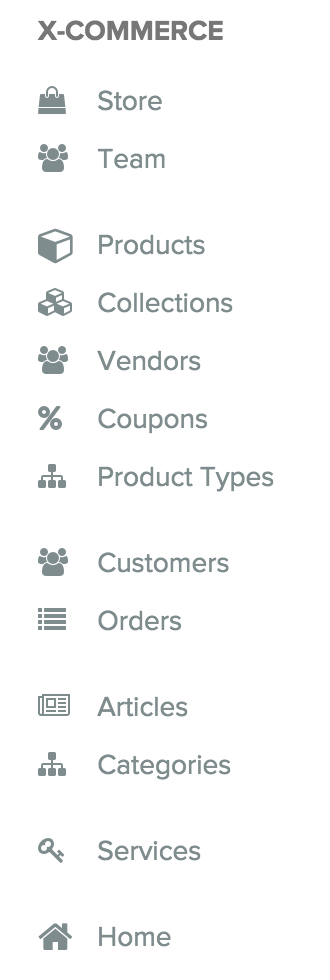
\includegraphics[width=0.2\linewidth]{images/chapter3/admin-nav.png}\hfill
\caption[Admin navbar]{Admin navbar}
\label{fig:design_page}
\end{figure}
The same philosophy to arrange everything in components has also been used for the client-side.
\newline
Following shows some screenshots of the pages that make up the admin interface:
\begin{figure}[htb]
\centering
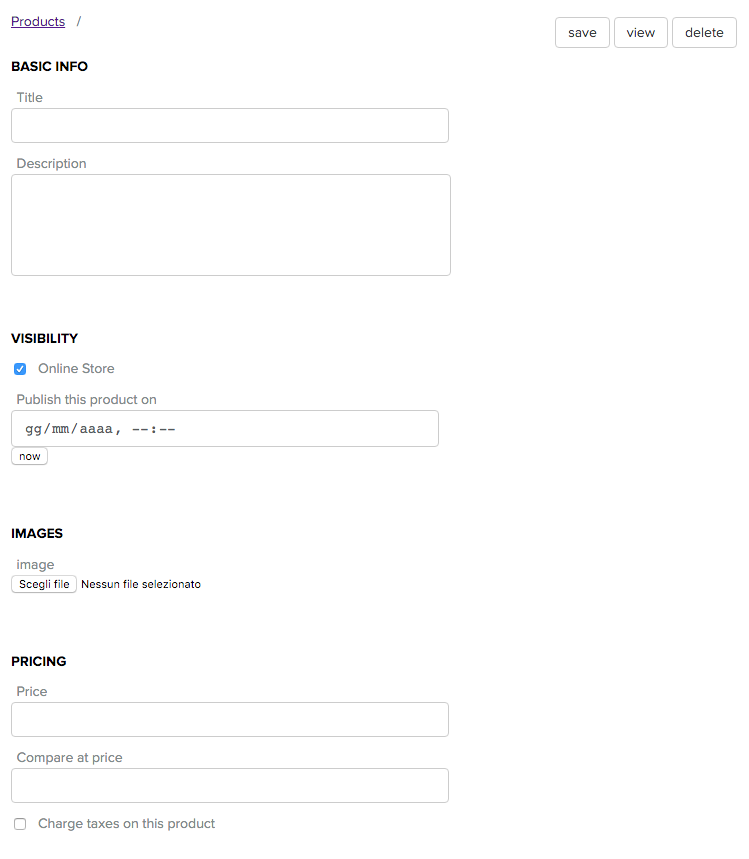
\includegraphics[width=1.0\linewidth]{images/chapter3/products-example.png}\hfill
\caption[page product first part form]{Page product example - first part form interface}
\label{fig:design_page}
\end{figure}

\begin{figure}[htb]
\centering
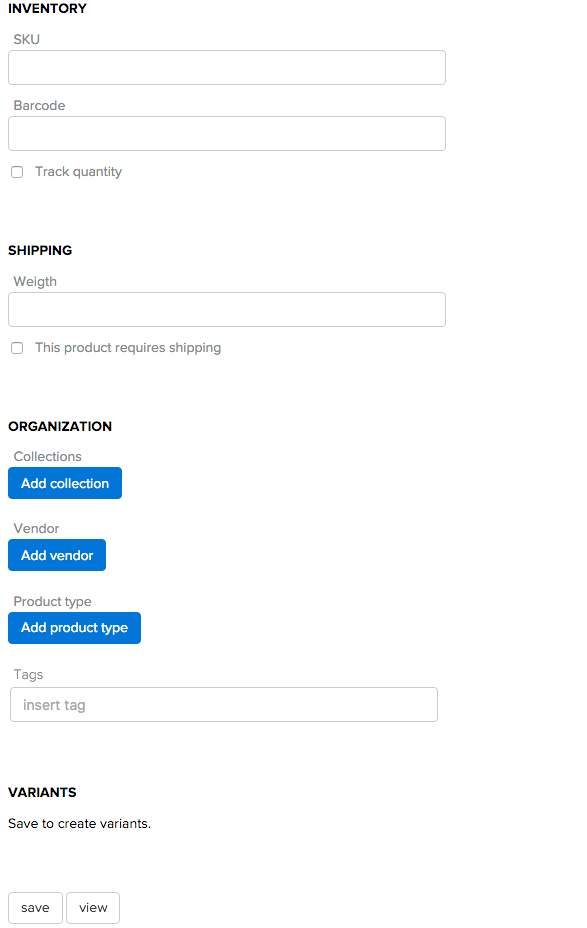
\includegraphics[width=1.0\linewidth]{images/chapter3/products-example1.png}\hfill
\caption[page product second part form]{Page product example - second part form interface}
\label{fig:design_page}
\end{figure}
%product page screenshot page product all browser
\begin{figure}[htb]
\centering
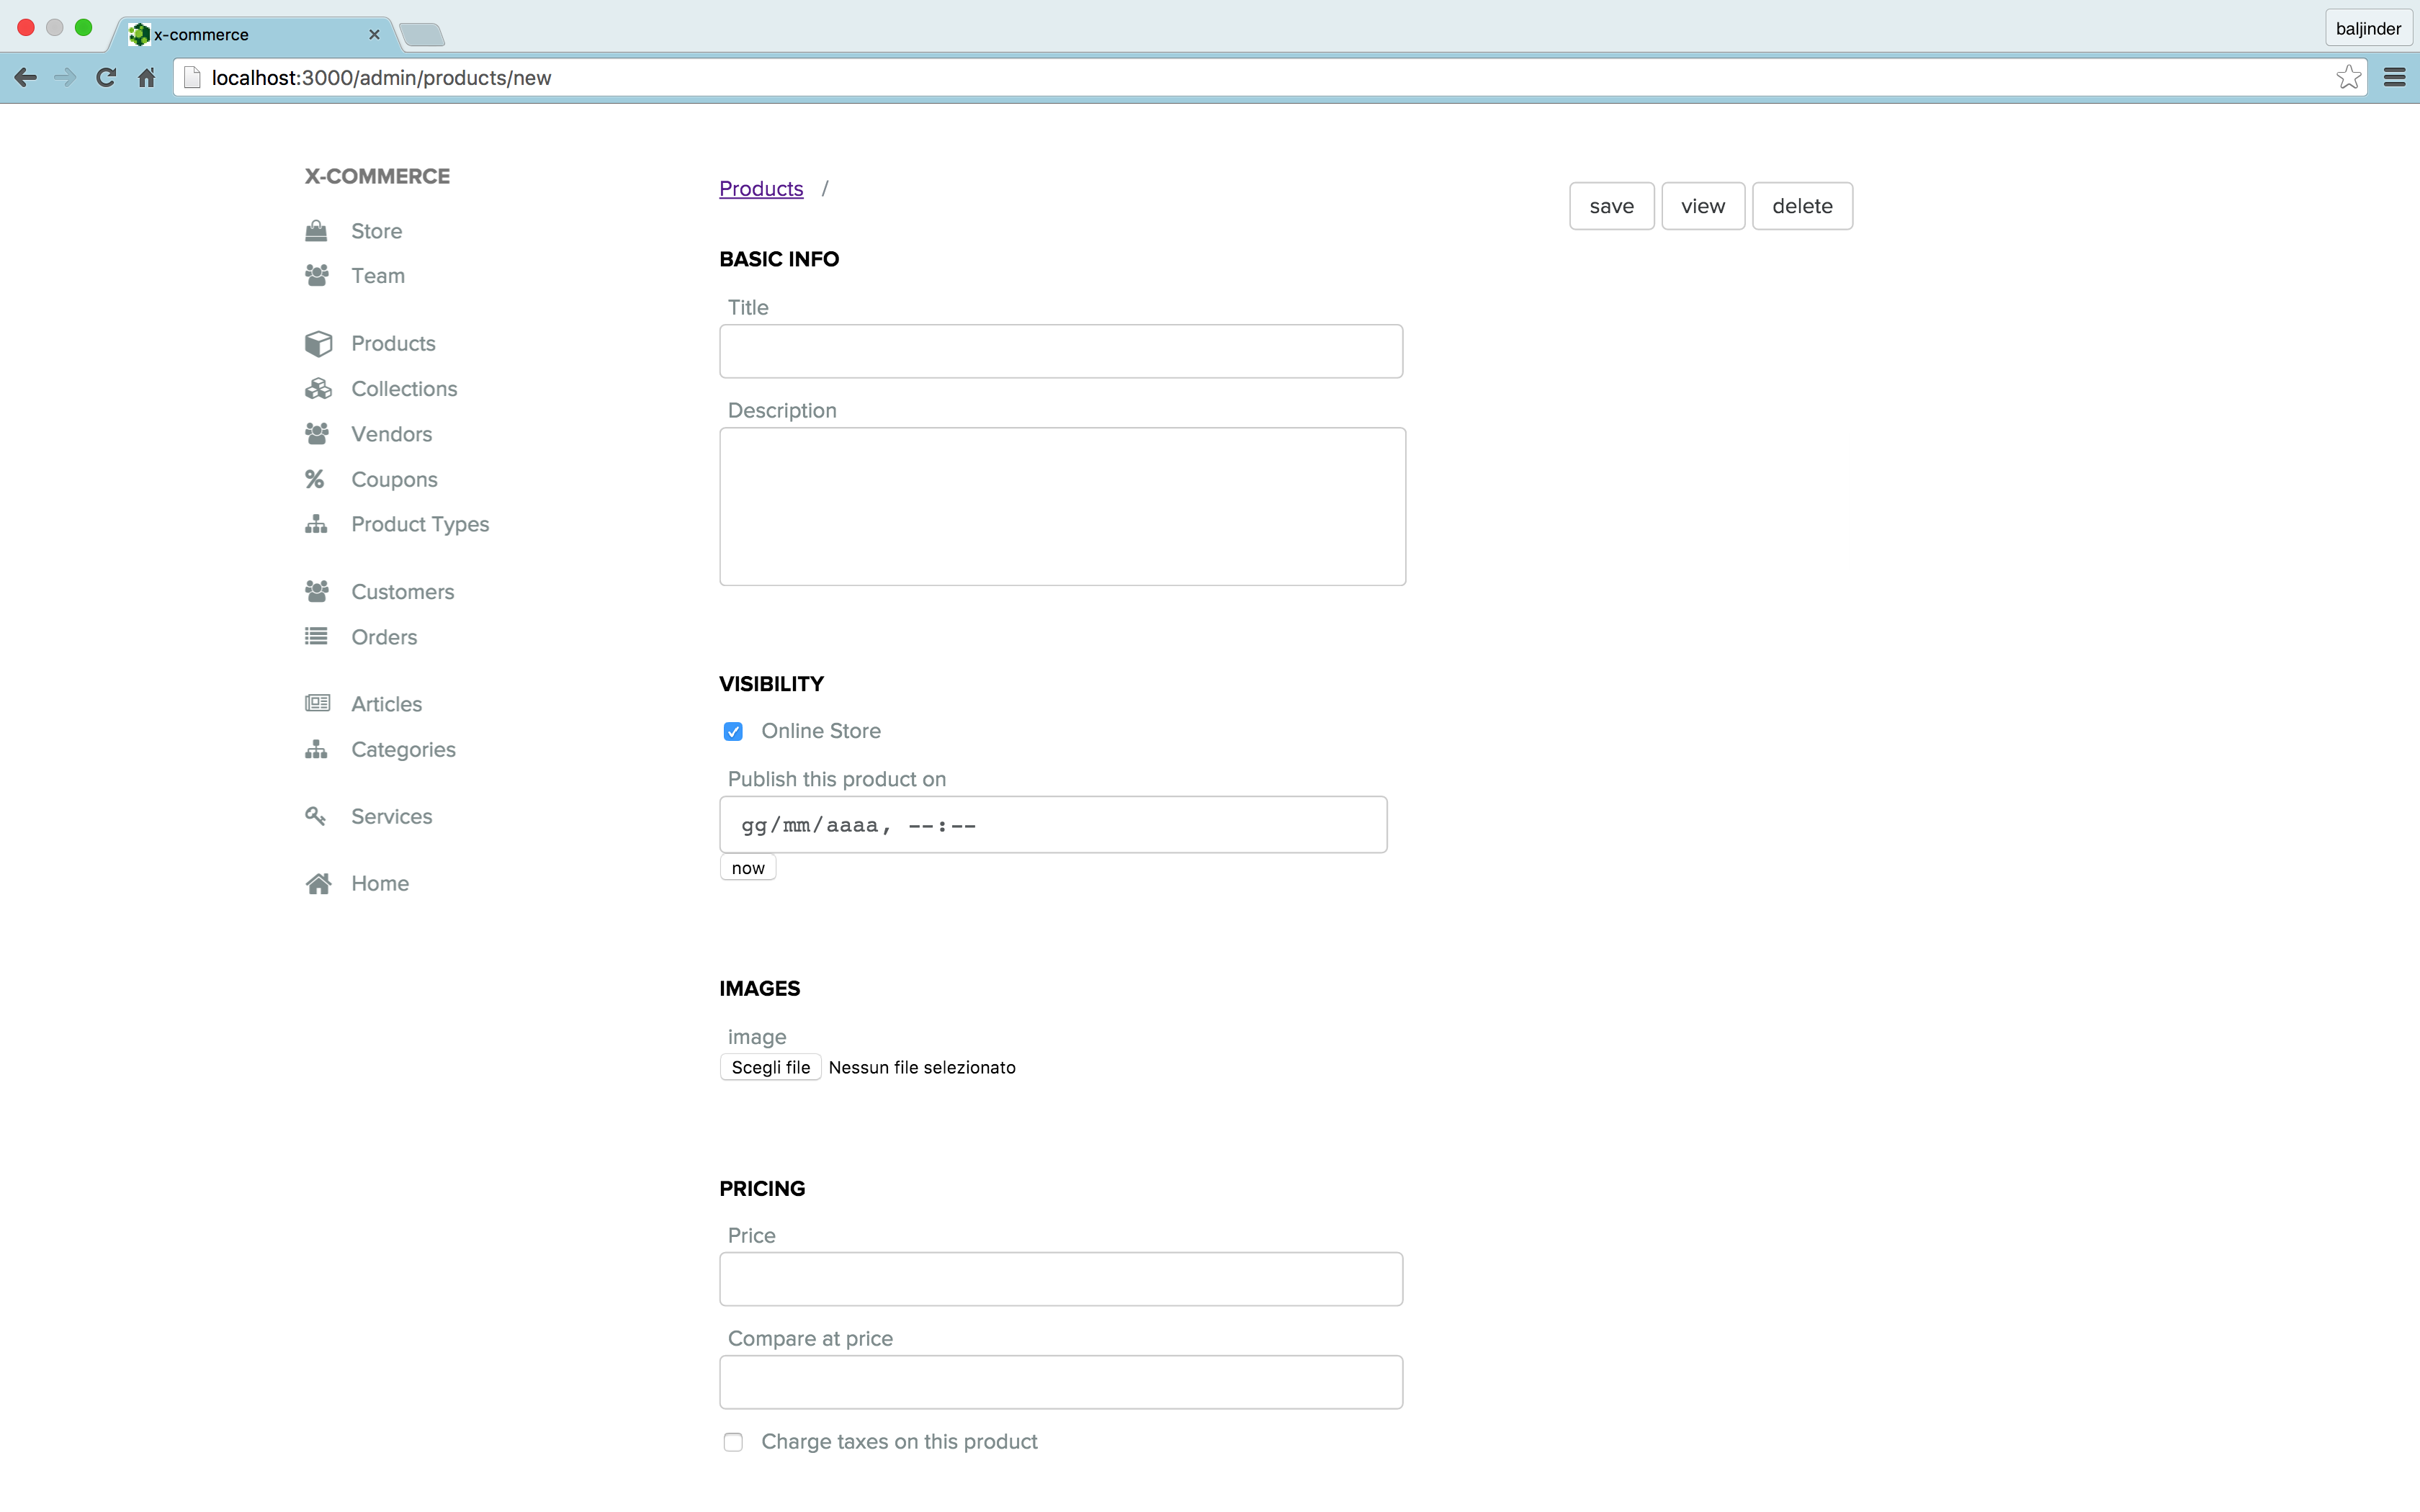
\includegraphics[width=1.0\linewidth]{images/chapter3/prod-part1-all.png}\hfill
\caption[page product first part form browser]{Page product example - first part form interface - Browser screenshot}
\label{fig:design_page}
\end{figure}
\begin{figure}[htb]
\centering
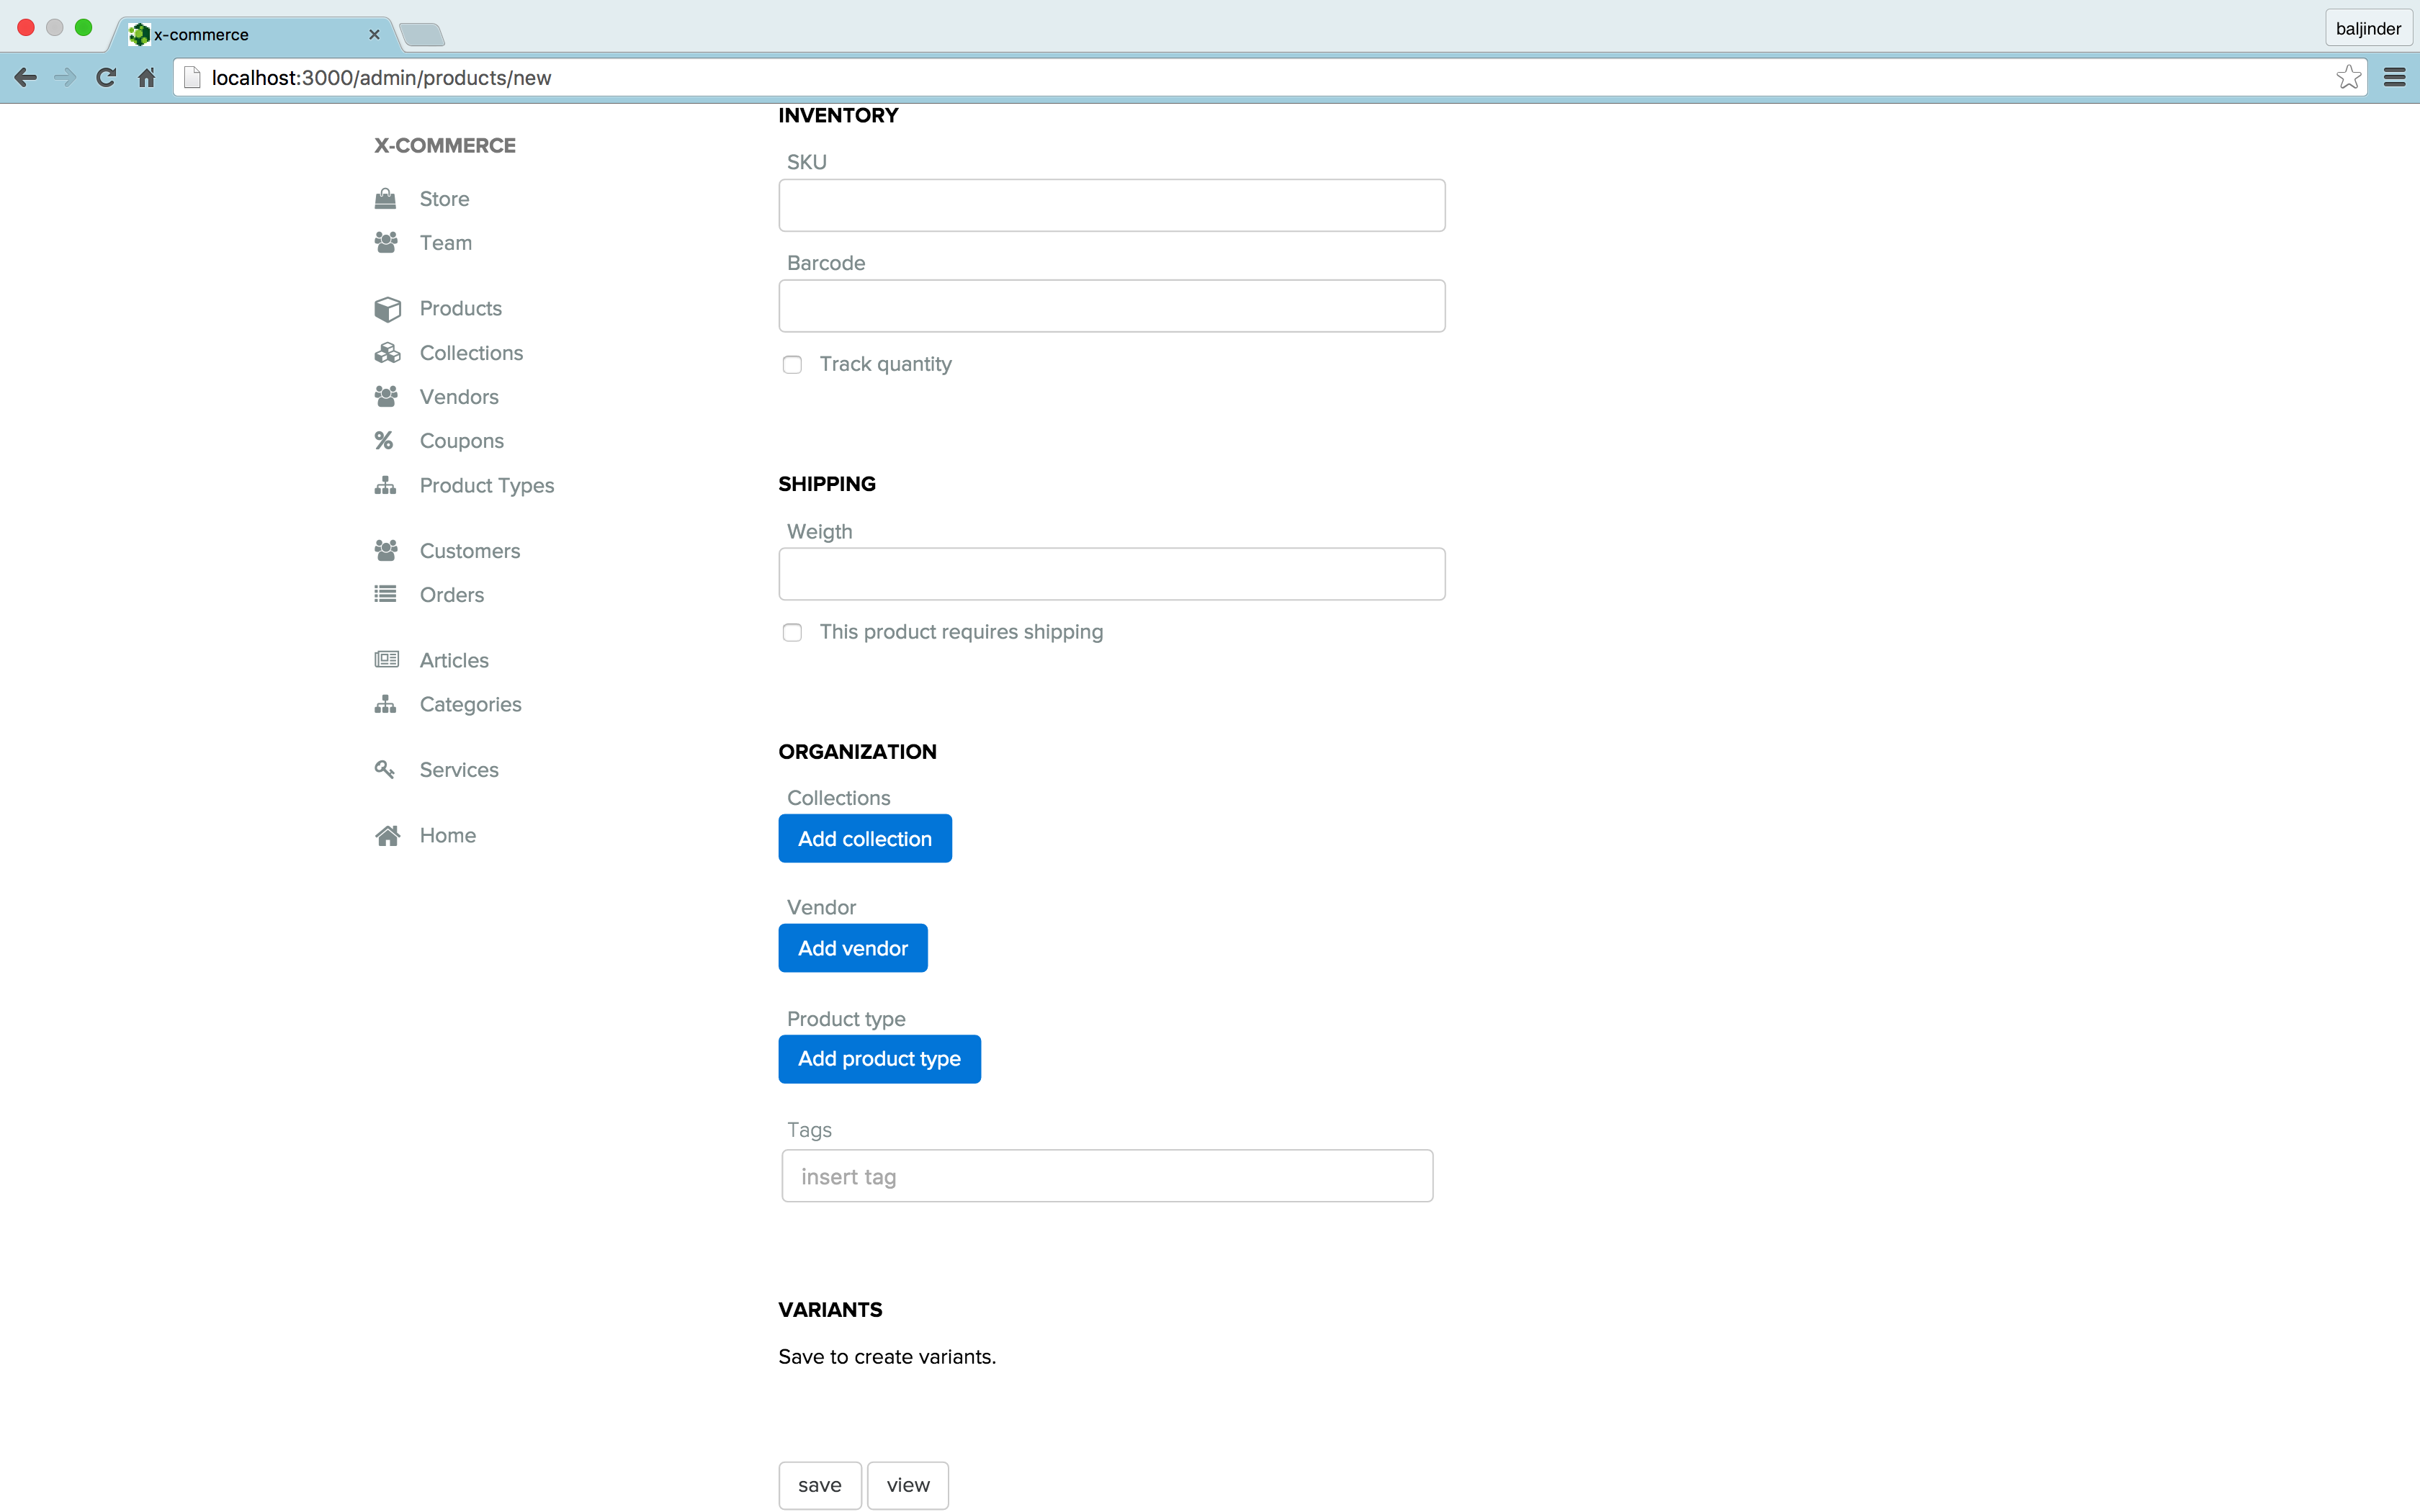
\includegraphics[width=1.0\linewidth]{images/chapter3/prod-part2-all.png}\hfill
\caption[page product second part form browser]{Page product example - second part form interface- Browser screenshot}
\label{fig:design_page}
\end{figure}
%page products example
\begin{figure}[htb]
\centering
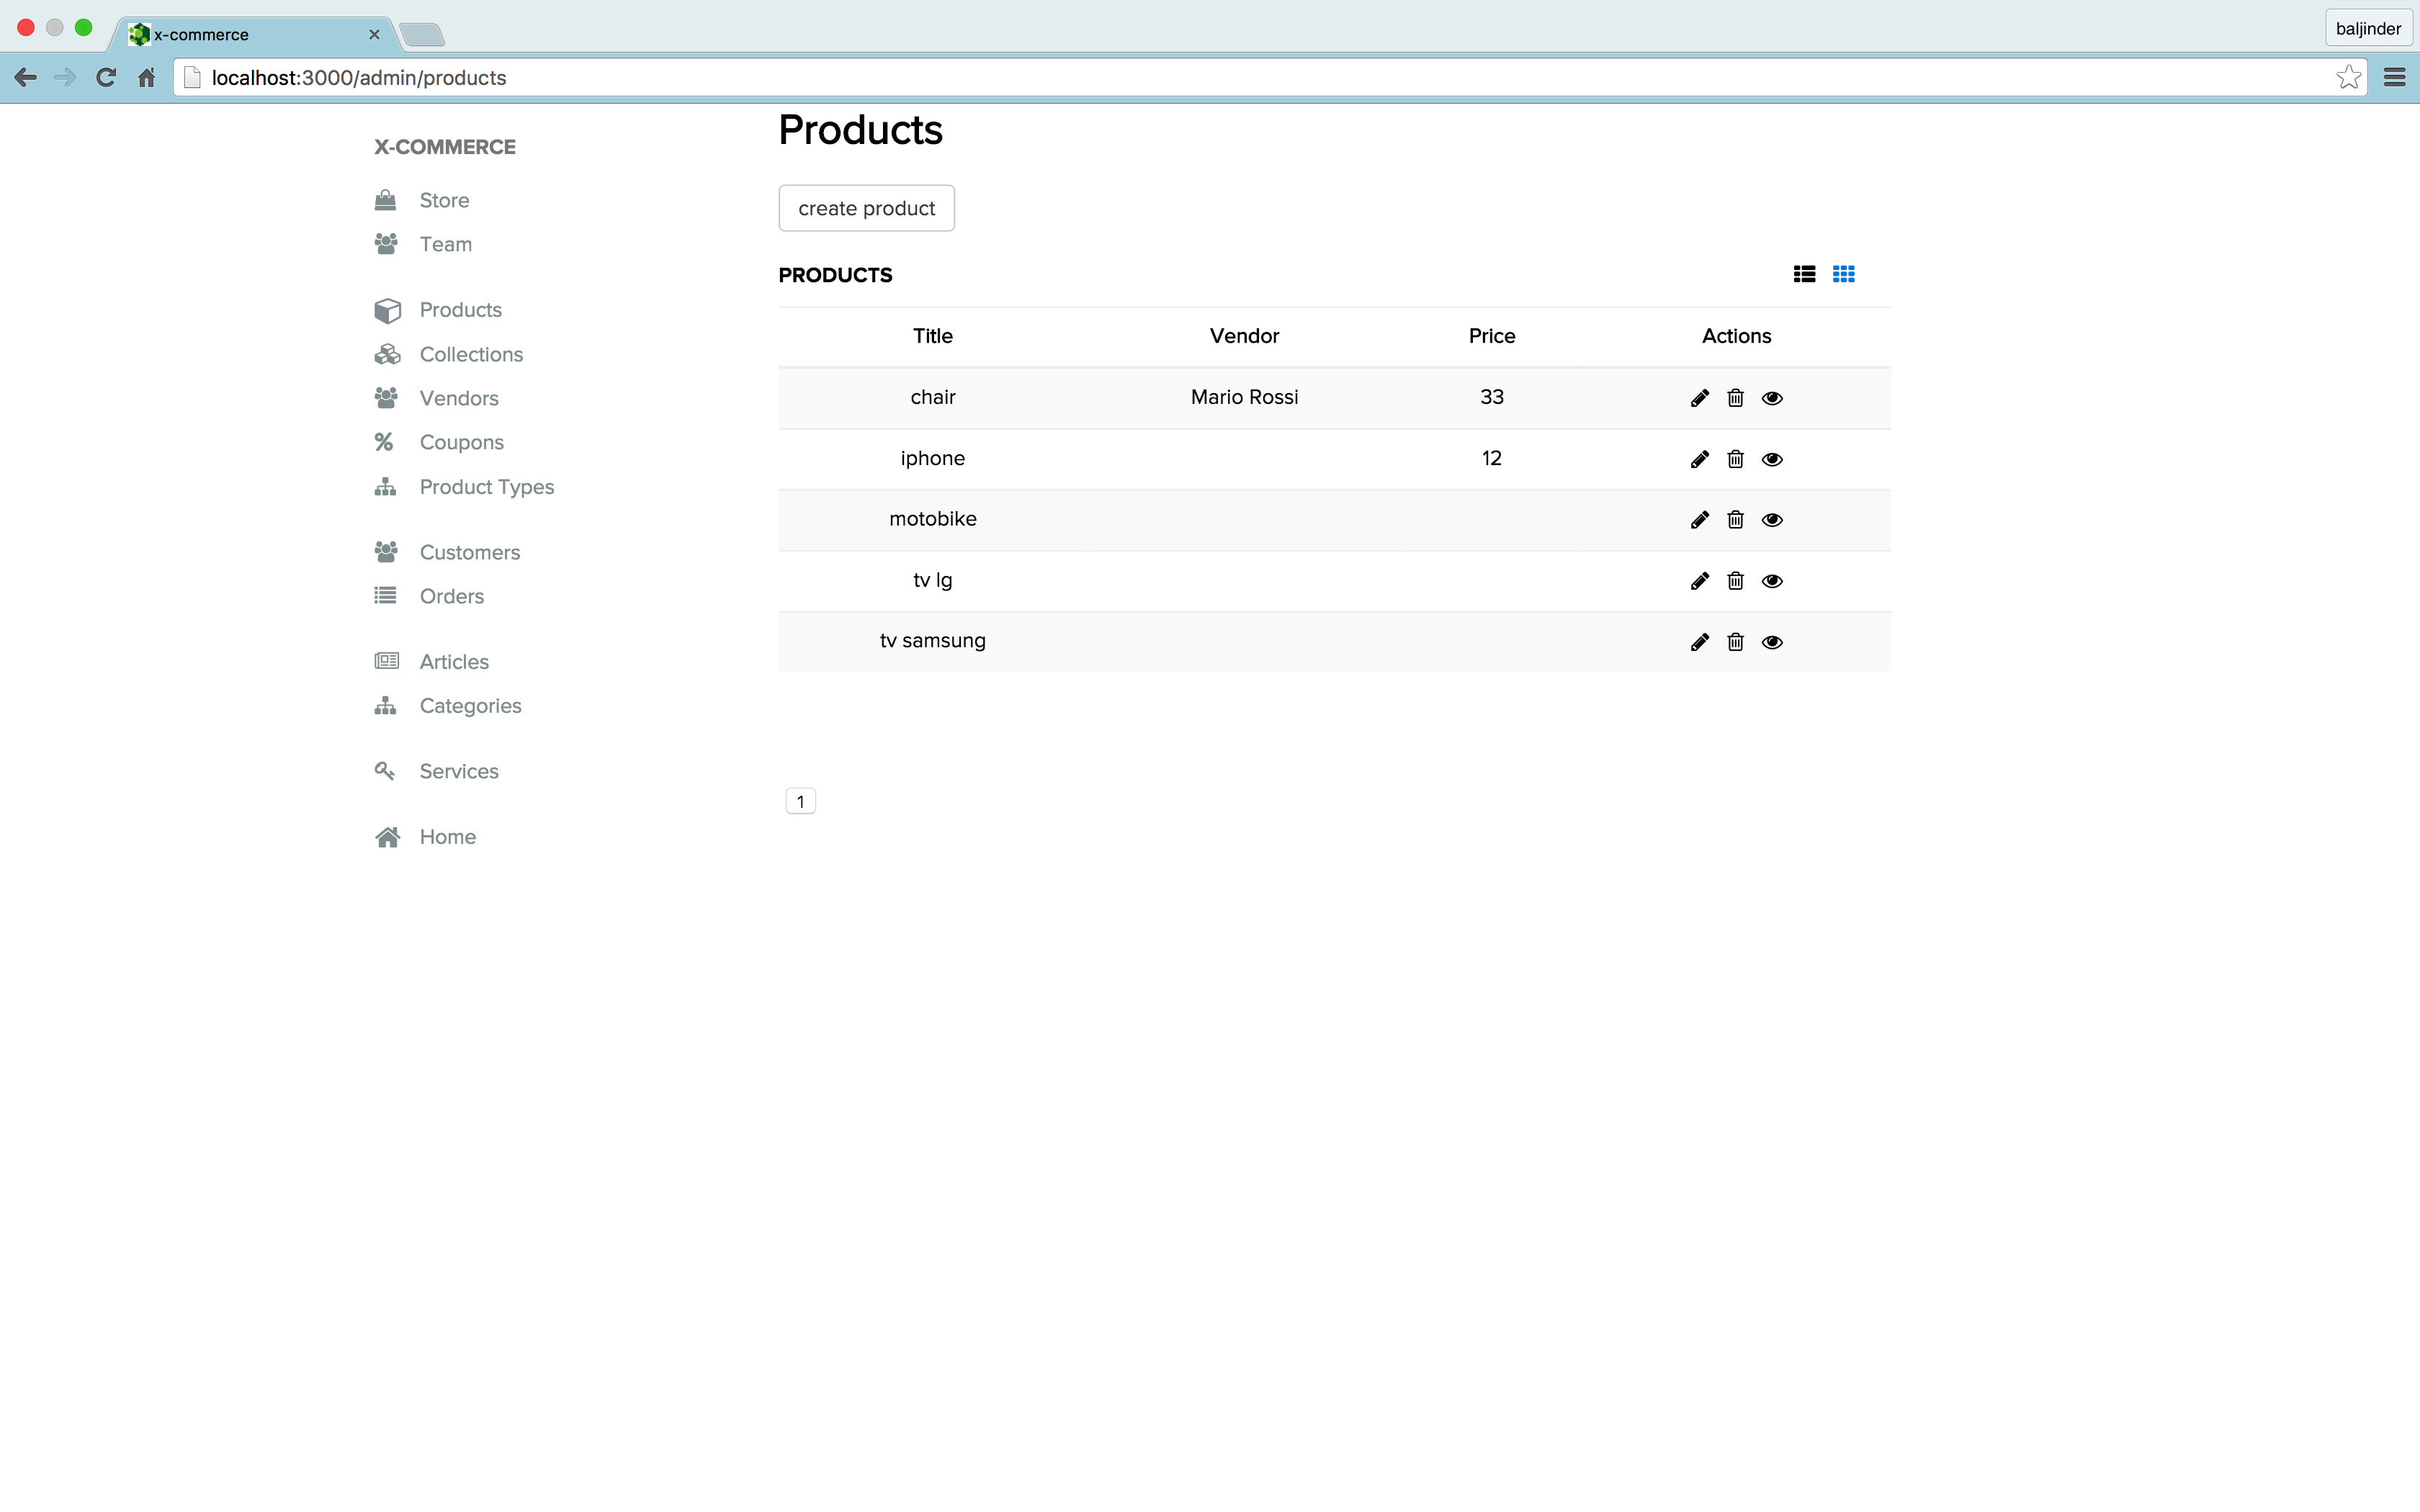
\includegraphics[width=1.0\linewidth]{images/chapter3/page-products-all.png}\hfill
\caption[page products example]{Page products example}
\label{fig:design_page}
\end{figure}
%page order example
\begin{figure}[htb]
\centering
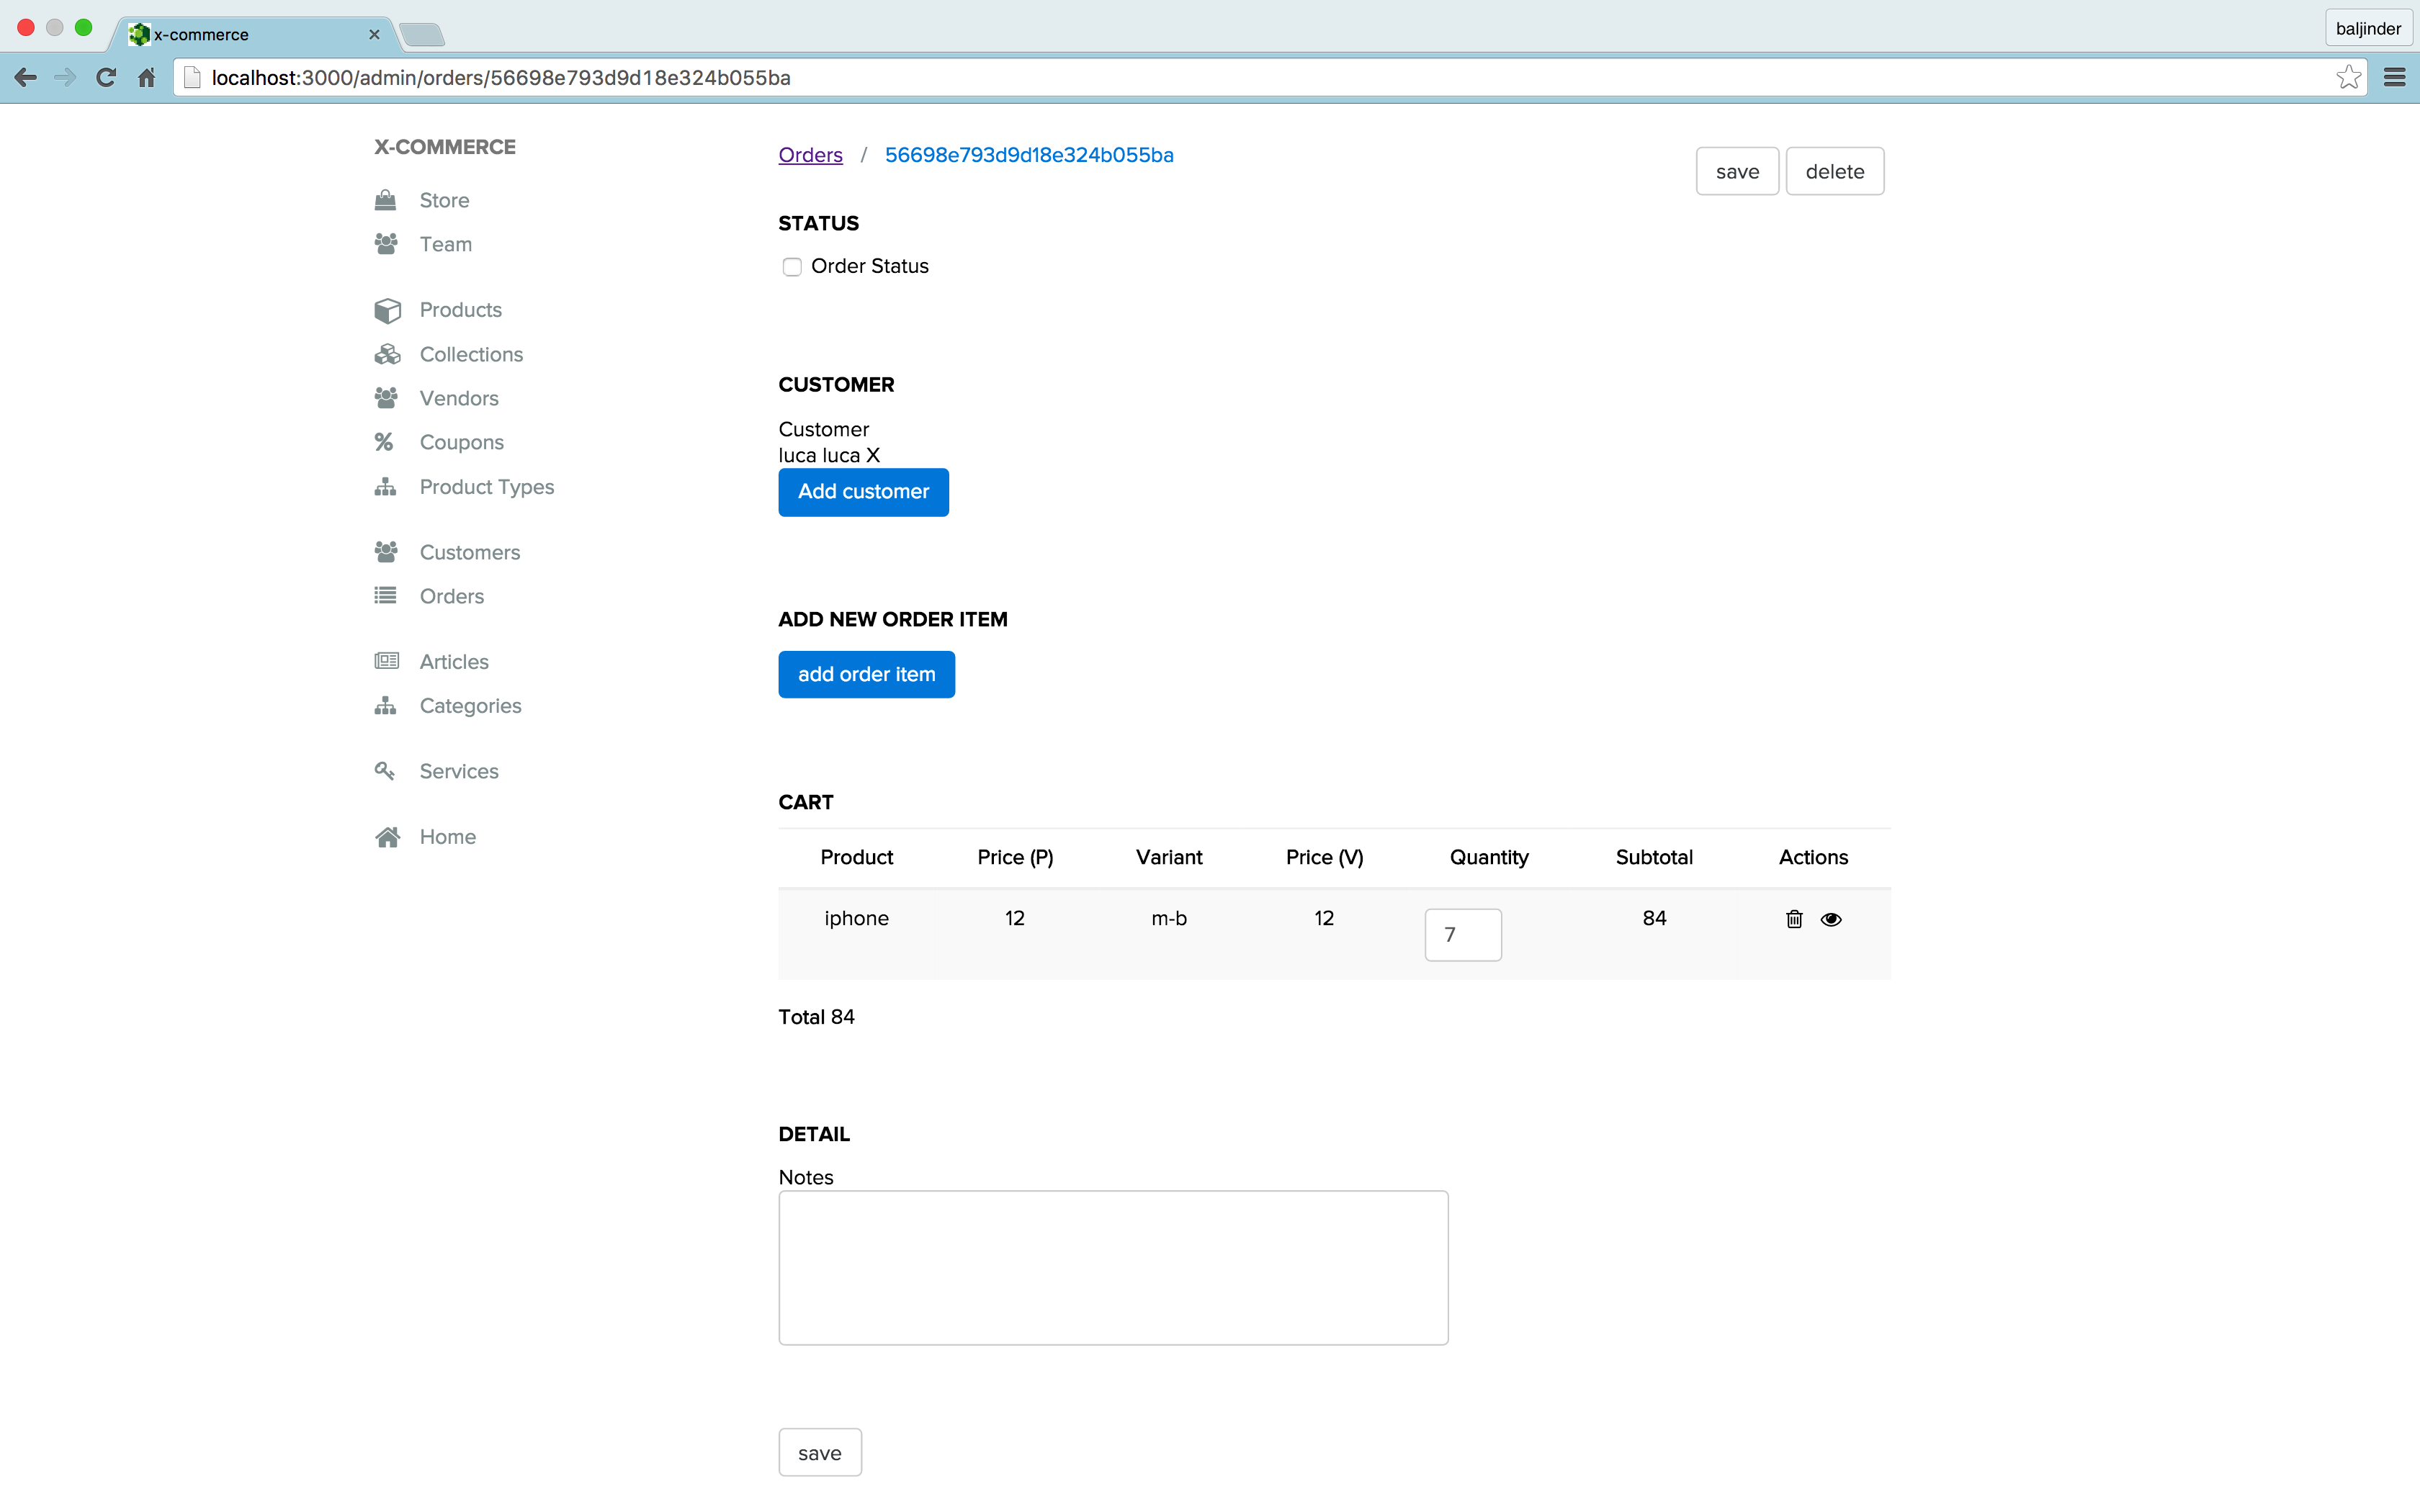
\includegraphics[width=1.0\linewidth]{images/chapter3/page-order-all.png}\hfill
\caption[page order example]{Page order example}
\label{fig:design_page}
\end{figure}
%page coupon example
\begin{figure}[htb]
\centering
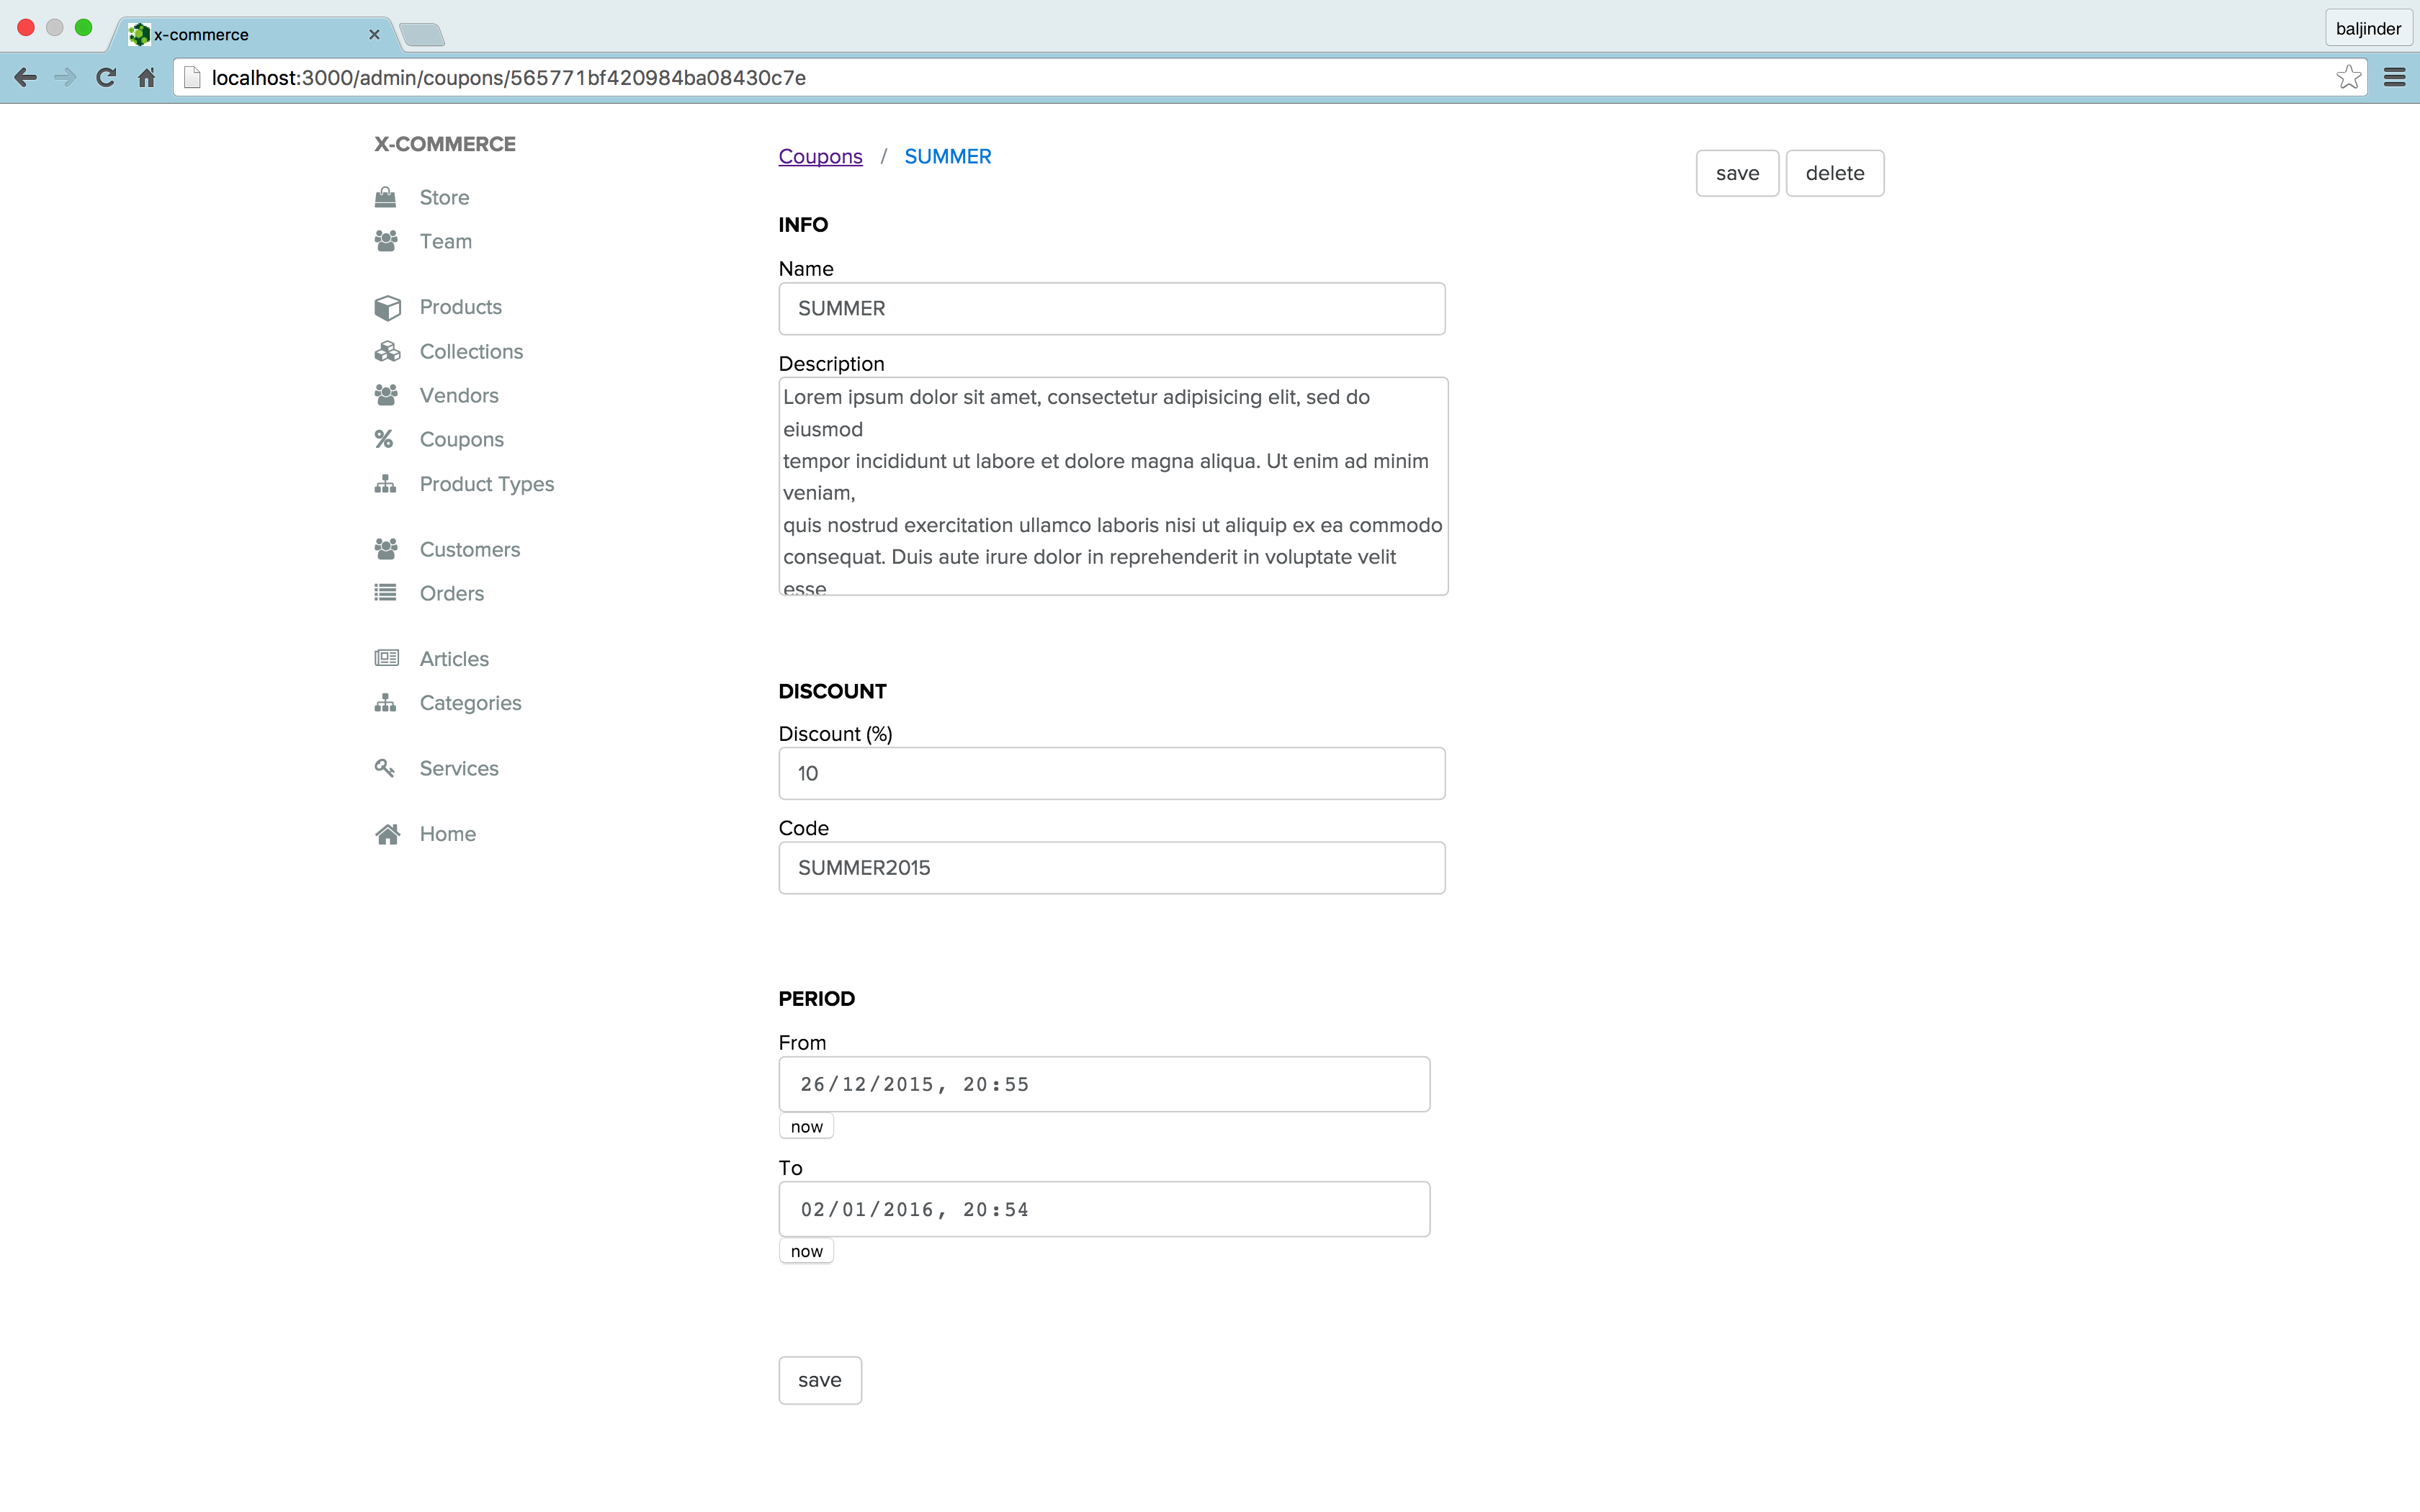
\includegraphics[width=1.0\linewidth]{images/chapter3/page-coupon-all.png}\hfill
\caption[page coupon example]{Page coupon example}
\label{fig:design_page}
\end{figure}
%page vendor example
\begin{figure}[htb]
\centering
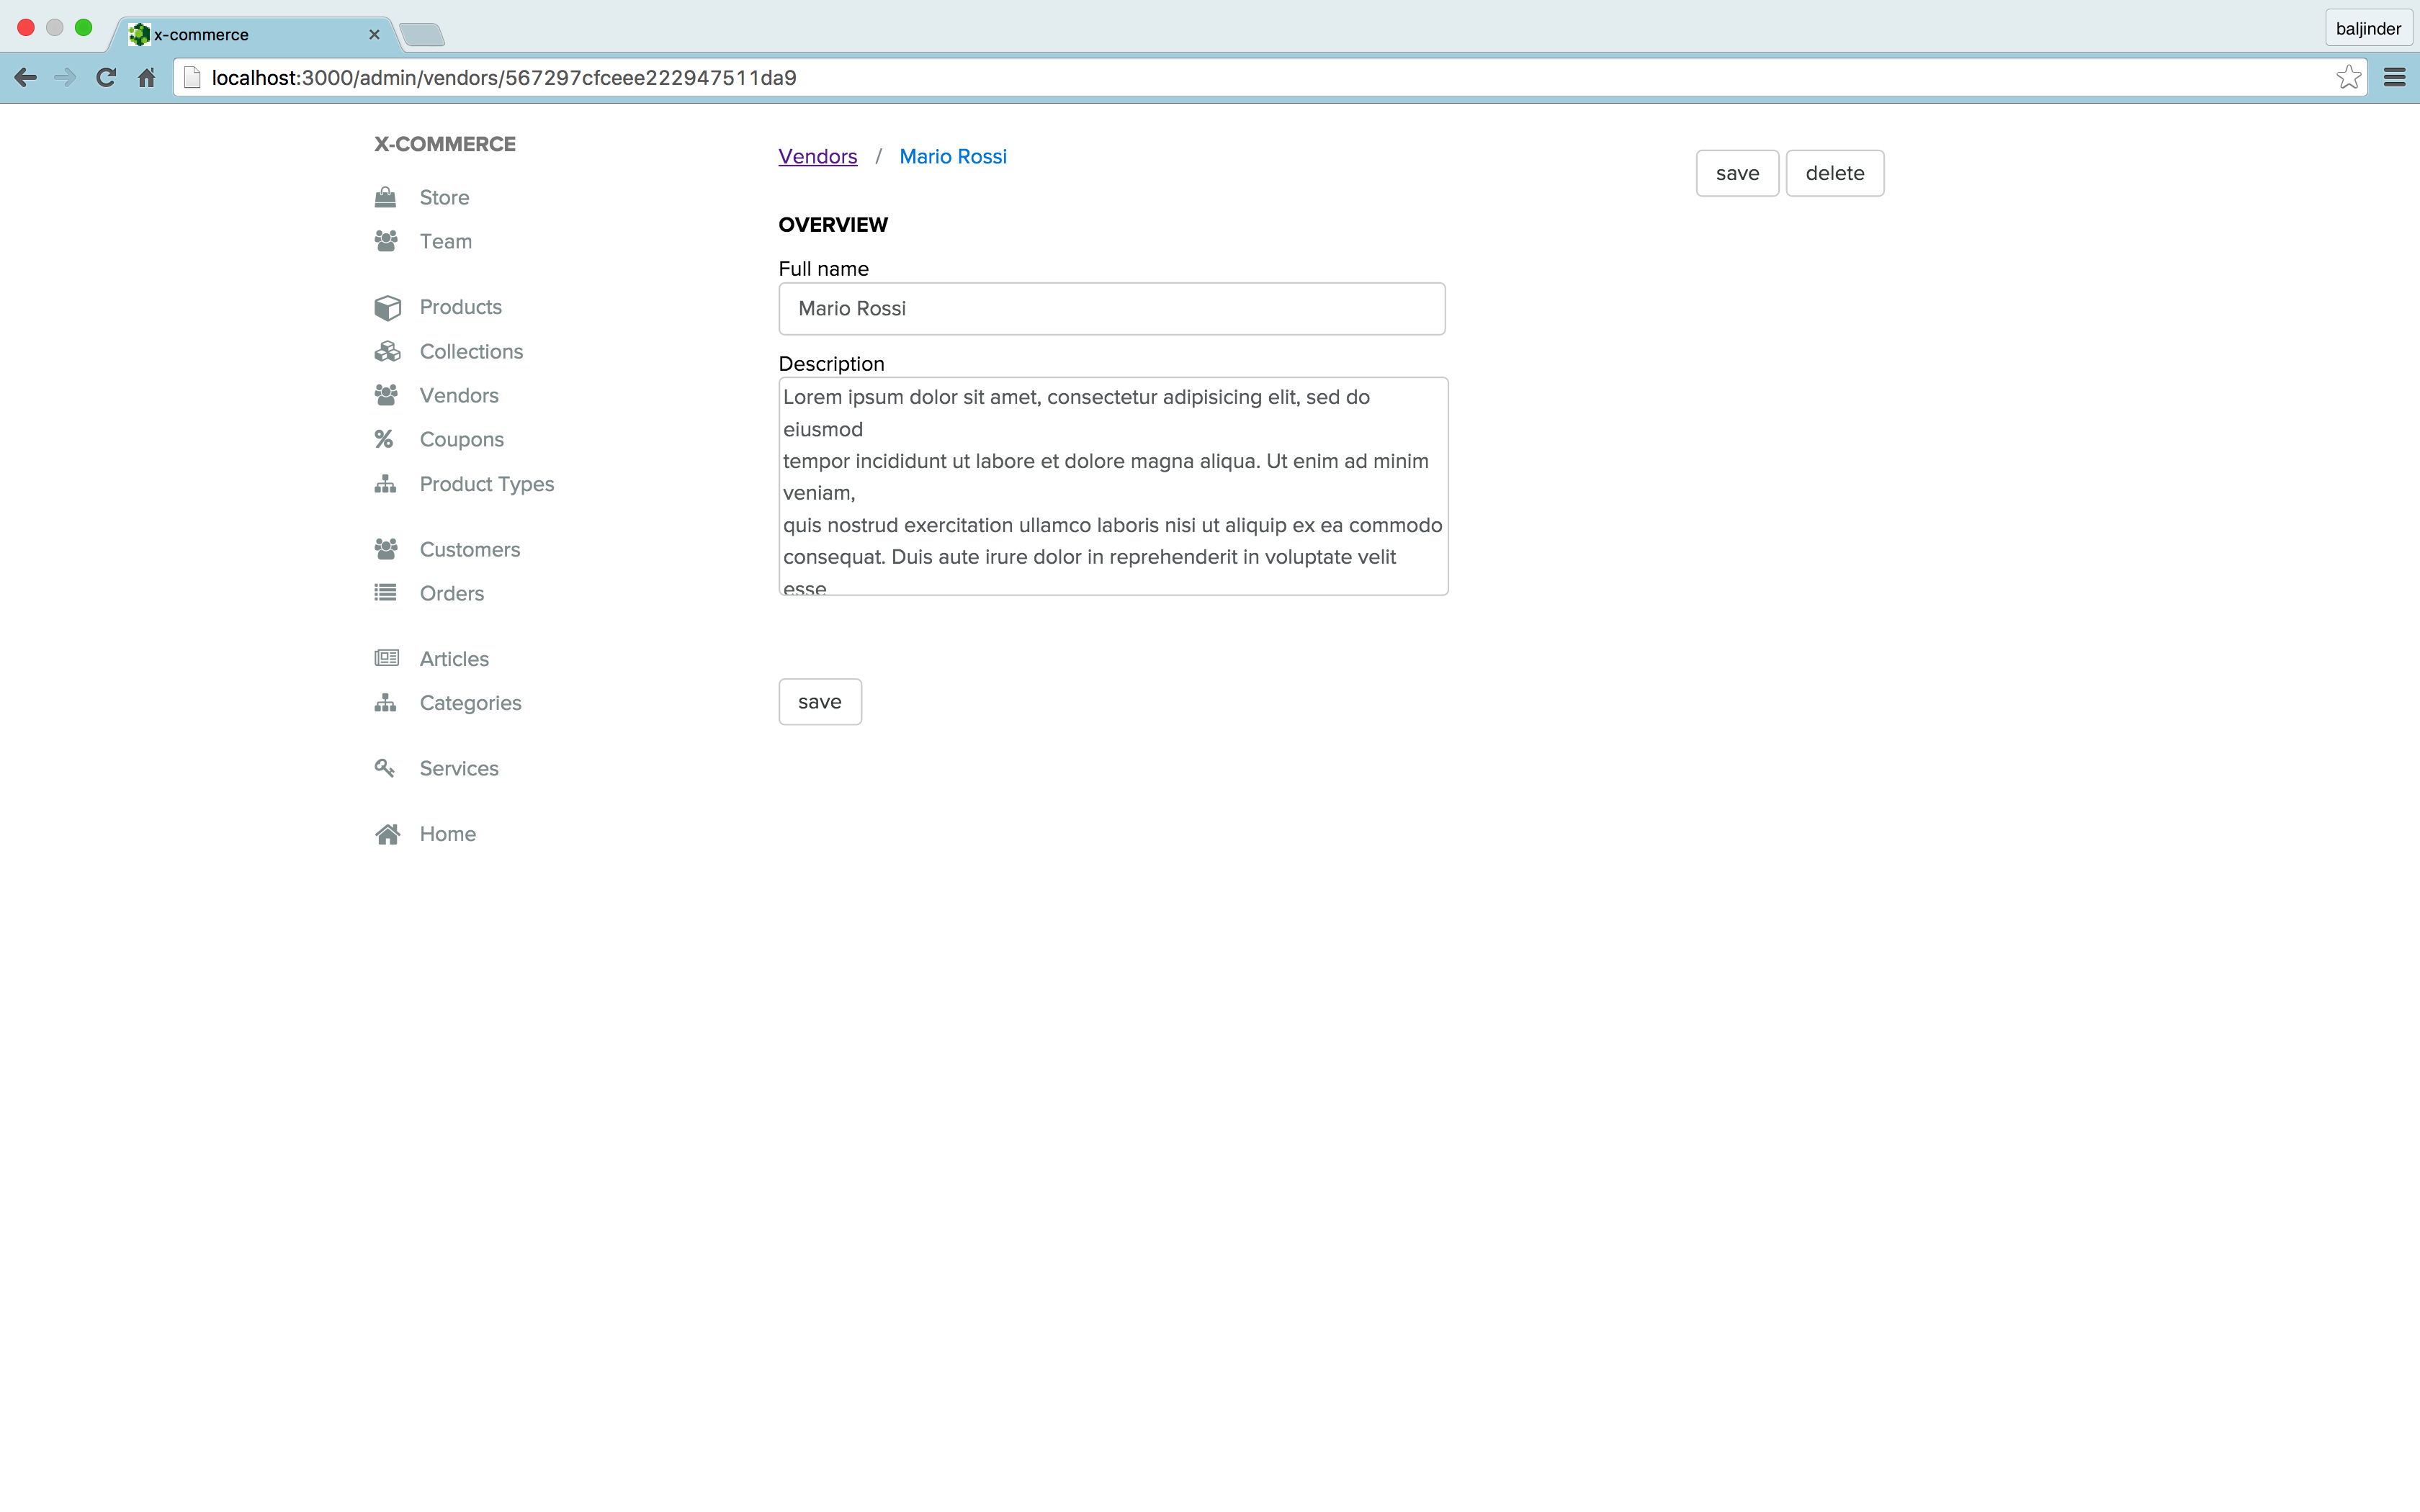
\includegraphics[width=1.0\linewidth]{images/chapter3/page-vendor-all.png}\hfill
\caption[page vendor example]{Page vendor example}
\label{fig:design_page}
\end{figure}